\documentclass[10pt]{article}
\usepackage{amsmath}
\usepackage{amssymb}
\usepackage{graphicx}
\usepackage{color} % for revision purposes only, may be not present in the final file
% cite package, to clean up citations in the main text. Do not remove.
% \usepackage{cite}
\usepackage{color}
\usepackage{indentfirst} %% LM: in order to indent the first paragraph of each section
\usepackage{url} %% LM: in order to include nice urls
\usepackage{booktabs} %% LM: nice tables...
\usepackage{subfigure} % LM: panels
\usepackage[authoryear,round]{natbib}
\bibliographystyle{apalike}
\usepackage{xr} % automatic cross-referencing
\externaldocument{Text_S2}
% Use doublespacing - comment out for single spacing
%\usepackage{setspace}
%\doublespacing

\topmargin 0.0cm
\oddsidemargin 0.5cm
\evensidemargin 0.5cm
\textwidth 16cm
\textheight 21cm

\usepackage[labelfont=bf,labelsep=period,justification=raggedright]{caption}


\makeatletter
\renewcommand{\@biblabel}[1]{\quad#1.}
\makeatother

\renewcommand{\thesubfigure}{(\Alph{subfigure})}
% Leave date blank
\date{}

\pagestyle{myheadings}
%% ** EDIT HERE **

%% ** EDIT HERE **
%% PLEASE INCLUDE ALL MACROS BELOW

%% END MACROS SECTION

% consistent edits between manuscript and rebuttal letter
%%
%% LaTeX source to reference manuscript changes in revision letters
%%
%% In the manuscript file:
%% 1. Include this file 
%%      %%
%% LaTeX source to reference manuscript changes in revision letters
%%
%% In the manuscript file:
%% 1. Include this file 
%%      %%
%% LaTeX source to reference manuscript changes in revision letters
%%
%% In the manuscript file:
%% 1. Include this file 
%%      \input{make-edits}
%% 2. Define manuscript modifications as
%%      \myedit{UniqueLabel}{Text to appear in manuscript and revision letter}
%%
%% In the revision letter file:
%% 1. Include the automatically updated modifications file
%%      \input{jobname.xtr}
%% 2. Include modified text with
%%      \myeditUniqueLabel
%%
%% Marc A. Suchard
%% 24-Jul-2006
%%

\newwrite\XTR
\AtBeginDocument{\immediate\openout\XTR\jobname.xtr}
\AtEndDocument{\immediate\closeout\XTR}

\newcommand{\myedit}[2]{ % first options is a label, second options is the text
\parbox{0em}{
\shipout\box1{
  \def\mynamea{myedit#1}
  \def\mynameb{\csname \mynamea\endcsname}
\write\XTR{
      \string\newcommand
{\csname myedit#1\endcsname}
}
\write\XTR{
         {``\expandafter\string#2''
         (pg.\string~\thepage)}
}
%\write\XTR{
%    (pg.\string~\thepage)
%}
}
%\hspace*{-1in}
}
%
%\def\thistext{\noexpand#2}
%  \immediate\write\XTR{
%   %     \begin{verbatim}
%        \thistext
%   %     \end{verbatim}
%  }
%\endgroup
%}
%\shipout\vbox{0}
%        \label{\expand\mylabel}
%        \thepage
%  \mylabel
%  \hspace*{-0em}
%  {\bf#2}
#2
}

\newcommand{\myeditblank}[2]{ % first options is a label, second options is the text
\parbox{1em}{
\shipout\box1{
  \def\mynamea{myedit#1}
  \def\mynameb{\csname \mynamea\endcsname}
\write\XTR{
      \string\newcommand
{\csname myedit#1\endcsname}
}
\write\XTR{
         {\expandafter\string#2
         (pg.\string~\thepage)}
}
%\write\XTR{
%    (pg.\string~\thepage)
%}
}
%\hspace*{-1in}
}
%
%\def\thistext{\noexpand#2}
%  \immediate\write\XTR{
%   %     \begin{verbatim}
%        \thistext
%   %     \end{verbatim}
%  }
%\endgroup
%}
%\shipout\vbox{0}
%        \label{\expand\mylabel}
%        \thepage
%  \mylabel
%  \hspace*{-1em}
%  {\bf#2}
}



%\newlength{\strikewidth}
%\newlength{\strikelength}
%\setlength{\strikewidth}{1pt}

%\newcommand{\remove}[1]{
%    \settowidth{\strikelength}{#1}
%    #1\hspace{-\strikelength}
%    \rule[0.5ex]{\strikelength}{\strikewidth}
%}

%\usepackage{ulem}
%\newcommand{\remove}[1]{\sout{#1}}
\newcommand{\remove}[1]{\hspace*{-1em}}

\newcommand{\add}[1]{
%        {\bf #1}
#1%\hspace*{0em}
}


%% 2. Define manuscript modifications as
%%      \myedit{UniqueLabel}{Text to appear in manuscript and revision letter}
%%
%% In the revision letter file:
%% 1. Include the automatically updated modifications file
%%      \input{jobname.xtr}
%% 2. Include modified text with
%%      \myeditUniqueLabel
%%
%% Marc A. Suchard
%% 24-Jul-2006
%%

\newwrite\XTR
\AtBeginDocument{\immediate\openout\XTR\jobname.xtr}
\AtEndDocument{\immediate\closeout\XTR}

\newcommand{\myedit}[2]{ % first options is a label, second options is the text
\parbox{0em}{
\shipout\box1{
  \def\mynamea{myedit#1}
  \def\mynameb{\csname \mynamea\endcsname}
\write\XTR{
      \string\newcommand
{\csname myedit#1\endcsname}
}
\write\XTR{
         {``\expandafter\string#2''
         (pg.\string~\thepage)}
}
%\write\XTR{
%    (pg.\string~\thepage)
%}
}
%\hspace*{-1in}
}
%
%\def\thistext{\noexpand#2}
%  \immediate\write\XTR{
%   %     \begin{verbatim}
%        \thistext
%   %     \end{verbatim}
%  }
%\endgroup
%}
%\shipout\vbox{0}
%        \label{\expand\mylabel}
%        \thepage
%  \mylabel
%  \hspace*{-0em}
%  {\bf#2}
#2
}

\newcommand{\myeditblank}[2]{ % first options is a label, second options is the text
\parbox{1em}{
\shipout\box1{
  \def\mynamea{myedit#1}
  \def\mynameb{\csname \mynamea\endcsname}
\write\XTR{
      \string\newcommand
{\csname myedit#1\endcsname}
}
\write\XTR{
         {\expandafter\string#2
         (pg.\string~\thepage)}
}
%\write\XTR{
%    (pg.\string~\thepage)
%}
}
%\hspace*{-1in}
}
%
%\def\thistext{\noexpand#2}
%  \immediate\write\XTR{
%   %     \begin{verbatim}
%        \thistext
%   %     \end{verbatim}
%  }
%\endgroup
%}
%\shipout\vbox{0}
%        \label{\expand\mylabel}
%        \thepage
%  \mylabel
%  \hspace*{-1em}
%  {\bf#2}
}



%\newlength{\strikewidth}
%\newlength{\strikelength}
%\setlength{\strikewidth}{1pt}

%\newcommand{\remove}[1]{
%    \settowidth{\strikelength}{#1}
%    #1\hspace{-\strikelength}
%    \rule[0.5ex]{\strikelength}{\strikewidth}
%}

%\usepackage{ulem}
%\newcommand{\remove}[1]{\sout{#1}}
\newcommand{\remove}[1]{\hspace*{-1em}}

\newcommand{\add}[1]{
%        {\bf #1}
#1%\hspace*{0em}
}


%% 2. Define manuscript modifications as
%%      \myedit{UniqueLabel}{Text to appear in manuscript and revision letter}
%%
%% In the revision letter file:
%% 1. Include the automatically updated modifications file
%%      \input{jobname.xtr}
%% 2. Include modified text with
%%      \myeditUniqueLabel
%%
%% Marc A. Suchard
%% 24-Jul-2006
%%

\newwrite\XTR
\AtBeginDocument{\immediate\openout\XTR\jobname.xtr}
\AtEndDocument{\immediate\closeout\XTR}

\newcommand{\myedit}[2]{ % first options is a label, second options is the text
\parbox{0em}{
\shipout\box1{
  \def\mynamea{myedit#1}
  \def\mynameb{\csname \mynamea\endcsname}
\write\XTR{
      \string\newcommand
{\csname myedit#1\endcsname}
}
\write\XTR{
         {``\expandafter\string#2''
         (pg.\string~\thepage)}
}
%\write\XTR{
%    (pg.\string~\thepage)
%}
}
%\hspace*{-1in}
}
%
%\def\thistext{\noexpand#2}
%  \immediate\write\XTR{
%   %     \begin{verbatim}
%        \thistext
%   %     \end{verbatim}
%  }
%\endgroup
%}
%\shipout\vbox{0}
%        \label{\expand\mylabel}
%        \thepage
%  \mylabel
%  \hspace*{-0em}
%  {\bf#2}
#2
}

\newcommand{\myeditblank}[2]{ % first options is a label, second options is the text
\parbox{1em}{
\shipout\box1{
  \def\mynamea{myedit#1}
  \def\mynameb{\csname \mynamea\endcsname}
\write\XTR{
      \string\newcommand
{\csname myedit#1\endcsname}
}
\write\XTR{
         {\expandafter\string#2
         (pg.\string~\thepage)}
}
%\write\XTR{
%    (pg.\string~\thepage)
%}
}
%\hspace*{-1in}
}
%
%\def\thistext{\noexpand#2}
%  \immediate\write\XTR{
%   %     \begin{verbatim}
%        \thistext
%   %     \end{verbatim}
%  }
%\endgroup
%}
%\shipout\vbox{0}
%        \label{\expand\mylabel}
%        \thepage
%  \mylabel
%  \hspace*{-1em}
%  {\bf#2}
}



%\newlength{\strikewidth}
%\newlength{\strikelength}
%\setlength{\strikewidth}{1pt}

%\newcommand{\remove}[1]{
%    \settowidth{\strikelength}{#1}
%    #1\hspace{-\strikelength}
%    \rule[0.5ex]{\strikelength}{\strikewidth}
%}

%\usepackage{ulem}
%\newcommand{\remove}[1]{\sout{#1}}
\newcommand{\remove}[1]{\hspace*{-1em}}

\newcommand{\add}[1]{
%        {\bf #1}
#1%\hspace*{0em}
}



\begin{document}

% Title must be 150 characters or less
\begin{flushleft}
{\Large
\textbf{Spatio-temporal Dynamics of Foot-and-Mouth Disease Virus in South America}
}
% Insert Author names, affiliations and corresponding author email.
\\
Luiz Max Carvalho$^{1\ast}$,
Nuno Rodrigues Faria$^{2,3}$,
Andres Perez$^{4}$,
Marc A.~Suchard$^{5,6}$,
Philippe Lemey$^{2}$,
Waldemir de Castro Silveira$^{7}$,
Andrew Rambaut$^{1,8,9}$,
Guy Baele$^{2}$
\\
\bf{1} Institute of Evolutionary Biology, University of Edinburgh, Edinburgh, United Kingdom.\\
\bf{2} Department of Microbiology and Immunology, Rega Institute -- KU Leuven, Leuven, Belgium.\\
\bf{3} Department of Zoology, University of Oxford, Oxford, United Kingdom.\\
\bf{4} University of Minnesota, Department of Veterinary Population Medicine, College of Veterinary Medicine, Saint Paul, USA.\\
\bf{5} Departments of Biomathematics and Human Genetics, David Geffen School of Medicine at UCLA, University of California, Los Angeles,  United States of America.\\
\bf{6} Department of Biostatistics, UCLA Fielding School of Public Health, University of California, Los Angeles,  United States of America.\\
\bf{7} Research and Development Division, Trimatrix Applied Biotechnology Ltd, Rio de Janerio, Brazil.\\
\bf{8} Fogarty International Center, National Institutes of Health, Bethesda, MD,  United States of America.\\
\bf{9} Centre for Immunology, Infection and Evolution at the University of Edinburgh, Edinburgh, United Kingdom.
$\ast$ E-mail: lm.carvalho@ed.ac.uk
\end{flushleft}
% Please keep the abstract between 250 and 300 words
\section*{Abstract}

\myedit{RefOneComOne}{
Although foot-and-mouth disease virus (FMDV) incidence has decreased in South America over the last years, the pathogen still circulates in the region and the risk of re-emergence in previously FMDV-free areas is a veterinary public health concern.
In this paper we merge epidemiological and genetic data to reconstruct spatiotemporal patterns and determinants of FMDV serotypes A and O dispersal in South America.
}

Key-words: Phylogeography, foot-and-mouth disease virus, South America, animal trade.

\section*{Introduction}

% \myedit{RefOneComOne}{}

Foot-and-mouth disease virus (FMDV) is a rapidly evolving picornavirus and the causative agent of foot-and-mouth disease (FMD), the most important disease of domestic and wild cloven-hoofed animals~\citep{Grubman2004}.
The virus can be classified in seven serotypes, three of which (A, O, and C) have circulated in South America.
Serotype A caused large epidemics throughout the Southern cone in recent years~\citep{Perez2001, Malirat2012}, while endemic circulation has been mostly limited to Venezuela~\citep{Malirat2012}.
Historically, serotype O has been the most prevalent serotype on the continent, but is now limited to areas in the Andean region, and in particular to Ecuador~\citep{Malirat2011a}.
\myedit{RefOneComTwo}{Serotype C on the other hand was last encountered in the continent in $1995$ in Brazil~\citep{Correa2002}.}
Historical reports suggest that FMDV arrived in South America in the late years of the 19th century with European colonization~\citep{Naranjo2013, Tully2008}. 
By the 1970s, FMD was widespread in the region, with several large-scale epidemics being caused by multiple subtypes~\citep{Saraiva2003}.
In South America, FMD control and eradication has traditionally been pursued using a combination of mass vaccination programs~\citep{Saraiva2004b} and control of animal movements from areas in which FMDV infection was suspected.
Over time, passive and active surveillance programs have, with different degrees of success, managed the early detection of FMDV.
In order to achieve complete eradication however, the strains involved in epidemics - especially those in previously FMDV-free areas - need to be accurately characterised.

Phylogenetic analyses have proven useful in recovering the transmission pathways from genetic data~\citep{Cottam2008a, Cottam2008b} and providing insight into the processes that drive re-emergence~\citep{DiNardo2011}.
More recently, molecular epidemiology tools have been used to infer the origin and evolutionary history of emerging strains in South America~\citep{Perez2001, Malirat2007, Malirat2011a, Malirat2011b, Maradei2013}.
However, as pointed out by Di Nardo, Knowles \& Paton~\citep{DiNardo2011}, a common feature of FMDV molecular epidemiology studies is that  joint evaluation of epidemiological, environmental and genetic data has usually been performed outside of an unified quantitative framework.
In the face of many sources of information, ranging from genetic data to environmental data on host distribution and outbreak counts, it's desirable to have a framework capable of integrating these sources of information coherently.
Phylodynamics combines population genetics and epidemiology to explicitly  model the interaction between ecological processes such as migration and selection and the shape of the phylogenies~\citep{Grenfell2004, Volz2013}.
Bayesian phylodynamics offers an attractive statistical framework to combine multiple sources of information while marginalizing over the topology space, thus accommodating phylogenetic uncertainty.
In particular, phylogeographic methods can be employed to understand viral spatial dynamics under explicit spatial diffusion models~\citep{Lemey2009}.
Further, an important research goal is to gain insight into the major determinants of FMDV spread in the continent.
Since animal movements constitute a major threat to eradication programs~\citep{Schley2009}, using animal trade data as predictors can be a valuable tool to understand the role of livestock commerce in the spread of FMDV.
For example, Nelson et al. ~\citep{Nelson2011} coupled swine trade data and genetic data to show that swine movements in the United States drove the spread of a novel influenza virus of the H1 subtype.

Here, we investigate the phylodynamic patterns of serotypes A and O in South America using all publicly available VP1 (1D) sequences for those serotypes in South America, sampled over a long time-period (1955-2010 for serotype A and 1994-2010 for serotype O) in nearly all south American countries affected by FMD.
We apply Bayesian phylogeographic methods to investigate the evolutionary dynamics of serotypes A and O in South America incorporating  genetic, spatial and epidemiological data such as livestock trade, geographic distances and vaccination coverage.
This flexible Bayesian phylogeographic framework allows for the testing of hypotheses concerning viral dispersal, while naturally accommodating phylogenetic uncertainty~\citep{Lemey2009, Faria2011}.
We use BEAST~\citep{Drummond2012} to infer time-structured phylogenies and reconstruct past population dynamics, to which we overlay vaccination and serotype-specific notification data.
To study the factors driving re-emergence, we use data on livestock trade and geographical distances as predictors for viral spatial diffusion and compare competing spatial dynamics models involving each predictor using recently developed methods. 

\section*{Results}

\section*{Discussion}

\subsection*{Sampling bias}

\section*{Methods}

\subsection*{Genetic and epidemiological data}

\textbf{Acquisition of genetic data.}
We retrieved all FMDV nucleotide sequences available from GenBank~\citep{Benson2013} from the National Center for Biotechnology Information (NCBI, \url{ http://www.ncbi.nlm.nih.gov/}) with more than $600$ bp.
This first step yielded $6, 907$ sequences which were then filtered to exclude all sequences that did not include the 1D (VP1) gene, resulting in $4, 507$ sequences being kept.
We then filtered for sequences from serotypes A and O, yielding $1051$ and $2350$ sequences, respectively.
Next, we excluded sequences that had been extensively passaged in cell culture and selected all sequences from South America (Argentina, Bolivia, Brazil, Colombia, Ecuador, Paraguay, Peru, Uruguay, Venezuela) for which information on country and year of isolation was available.

This resulted in $185$ sequences (from eight countries) for serotype A and $215$ sequences (nine countries) for serotype O, covering time spans of $58$ ($1955$-$2013$) and $53$ (1958-2011) years, respectively (see Tables~\ref{stab:sequences_A} and~\ref{stab:sequences_O} for details).
We aligned each data set using the MAFFT~\citep{Katoh2002} algorithm implemented in the Geneious~\citep{Kearse2012} software package.
After a preliminary phylogenetic analysis (see below), an early serotype A sequence (Venezuela 1951) was excluded because its root-to-tip divergences was incompatible with its sampling date~\citep{Rambaut2016}.
For serotype O, five sequences were excluded under the same criteria (Table~\ref{stab:exclseqs}).
The final data sets had $184$ and $210$ sequences for serotypes A and O, respectively.

\textbf{Acquisition of trade data.}
Data on animal trade were obtained from the FAO database (\url{http://faostat.fao.org/}).
We retrieved data on the \textit{detailed trade matrix} for cattle, pigs and sheep (number of live animals exchanged) covering the period from $1986$ to $2009$, for each of the nine countries.
Serotype-specific outbreak notifications were obtained from FMD Bioportal (\url{http://fmdbioportal.ucdavis.edu:8080/}).

\textbf{Data availability.} All the data used in this paper, BEAST XML files as well as code to produce many of the plots/analyses are hosted at~\url{https://github.com/maxbiostat/FMDV_AMERICA}.

\subsection*{Phylogenetic Analysis}

We assume a general time reversible (GTR)~\citep{Tavare1986} model of sequence evolution, along with gamma-distributed rate heterogeneity (4 categories) for all our analyses.
We conducted an initial analysis of the two data sets described, employing PhyML~\citep{Guindon2003} to obtain maximum likelihood phylogenies which we then used in conjunction with Tempest~\citep{Rambaut2016} to produce root-to-tip divergence (RDV) plots and identify discrepant sequences (see ~\cite{Rambaut2016} for details).


% From here on we take a Bayesian approach to testing evolutionary hypotheses while accommodating phylogenetic uncertainty. 
Having identified considerable rate variation among branches we used the Bayesian Evolutionary Analysis by Sampling Trees (BEAST)~\citep{Drummond2012,Suchard2018} software package to infer time-structured phylogenies under relaxed clock models~\citep{Drummond2006}, employing the BEAGLE~\citep{Ayres2012} library to gain computational efficiency.

% \subsection*{Quantifying temporal and spatial signal} 
% 
% To assess the temporal signal for each serotype, we use the approach described in Faria et al.~\citep{Faria2012} and Baele et. al~\citep{Baele2012} and compare the marginal likelihoods of a dated-tips model and a contemporaneous-tips model by calculating Bayes Factors (BF)~\citep{Suchard2001, Suchard2005} (see Spatial Model Selection for details).
% We follow Kass and Raftery (1995)~\citep{KassRaftery1995} and consider a log BF$>$3 to be indicative of decisive support for the hypothesis of temporal structure.
% 
% We quantify spatial signal using Bayesian tip-association tests, implemented through the BaTS software package~\citep{Parker2008}.
% To detect phylogeny-location association, we assign each sequence to its country of origin and compute association index (AI) and parsimony score (PI) using BaTS on a subset of 1000 samples from the posterior distribution of topologies.
% We obtain a null distribution for each statistic (AI and PI), against which the observed indices are compared and significance is assessed.
% Additionally, we compute the monophyletic clade (MC) size for each state (country), as a local indicator of phylogeny-trait association for each state (country).
% Please see Text S2 for further details on the BaTs analyses.

\subsection*{Spatio-temporal Dynamics}

\textbf{Effective population size reconstruction}.
We employed the Skygrid coalescent model~\citep{Gill2012} to reconstruct that past population dynamics of both serotypes.
Skygrid necessitates the specification of a cutoff value, $K$, commensurate with the age of the root.
We have used $K = 100$ years for both data sets as a conservative estimate of the maximum age of the most recent common ancestor (mRCA) of the sampled sequences. 

\textbf{Phylogeography}.
To study the influence of different epidemiological predictors on viral diffusion through space, we used information on the trade of live cattle, pigs and sheep divided in three periods ($1986-1995$ , $1996-2004$, $2005-2013$).
Additionally, to assess the influence of over (under) sampling, we also included absolute differences in sequence (samples) numbers between locations as a predictor of flow (see the appendix in~\cite{Lemey2014} for a discussion).

\subsection*{Model selection}

In order to compare the performance of combinations of sequence evolution (Markov) and relaxed clock models for each data set
% (see Text S2)
, we use state-of-the-art marginal likelihood estimators, namely generalised stepping-stone sampling (SS)~\citep{Baele2015} implemented in BEAST~\citep{Suchard2018}.
% In this study we exploit recent developments in Bayesian model selection~\citep{Baele2012, Baele2013a, Baele2013b, Baele2013c, Baele2015}, as implemented in the BEAST software program~\citep{Suchard2018}.
Following a preliminary Skygrid analysis, we chose the constant population size coalescent parametric model and its associated working prior as the tree prior for these comparisons.
% Specifically, we perform accurate estimation of the (log) marginal likelihood using path sampling (PS)~\citep{Lartillot2006} and stepping-stone sampling (SS)~\citep{Xie2011}, two computationally demanding approaches that yield accurate estimates of model fit while accommodating phylogenetic uncertainty.
% Using these (log) marginal likelihoods, it's possible to calculate Bayes Factors, which provide a measure of the relative performance of each model. 
% We have estimated all the (log) marginal likelihoods in this study using 64 power posteriors, which were each run for 2 million iterations, taking up to 4 weeks of (wall time) computation for each model under evaluation. 
% Using PS and SS, we first compare different demographic priors and clock models (see Supplementary Text S2) for both serotypes. 
% For more details on these model selection procedures please see Supplementary Text S2.


% To test the influence of different epidemiological predictors on viral diffusion through space, we use to parameterize priors for the CTMC rate matrix.
% We normalize the numbers of live animals exchanged between countries to a mean and coefficient of variation of $1$ and use these as prior expectations in BEAST (see~\citep{Lemey2009}, pg. 14 and the Appendix in~\citep{Carvalho2013}).  
% We compare these predictors to a distance-informed prior~\citep{Lemey2009}, which represents a scenario where flow occurs as a function of the inverse of the geographic distances between locations.
% Finally, we compare all predictors against an equal-rates gamma prior, which considers~\textit{a priori} a scenario where there is no preferential spread among different countries~\citep{Nelson2011}.
\section{Software versions and computer codes}

\section*{Acknowledgments}
The authors would like to thank Ant\^onio Mendes (PANAFTOSA) for clarifications regarding the vaccination data, Matthew Hall (Oxford) and Oliver Pybus (Oxford) for insightful contributions and Miguel Carvalho, Felipe Figueiredo (PROCC) and Mauricio Oliveira (UFRJ) for operational support.
We acknowledge the support of the National Evolutionary Synthesis Center (NESCent) through a working group (Software for Bayesian Evolutionary Analysis).

\emph{Funding:} The research leading to these results has received funding from the European Union Seventh Framework Programme [FP7/2007-2013] under Grant Agreement no. 278433-PREDEMICS and ERC Grant agreement no. 260864.
This work was also supported by National Institutes of Health grants R01 HG006139 and National Science Foundation grants DMS 1264153.

\emph{Conflict of Interest:} none declared

\newpage
\bibliography{FMDV_AMERICA}
% \newpage
\section*{Figure Legends}
\newpage
\section{Figures and Tables}
%%%%%%%%%%%%%%%%%%%%%%%%%%
%%%%%%%%%%%%%%%%%%%%%%%%%%
% \begin{figure}[!ht]
% \begin{center}
% \subfigure[A]{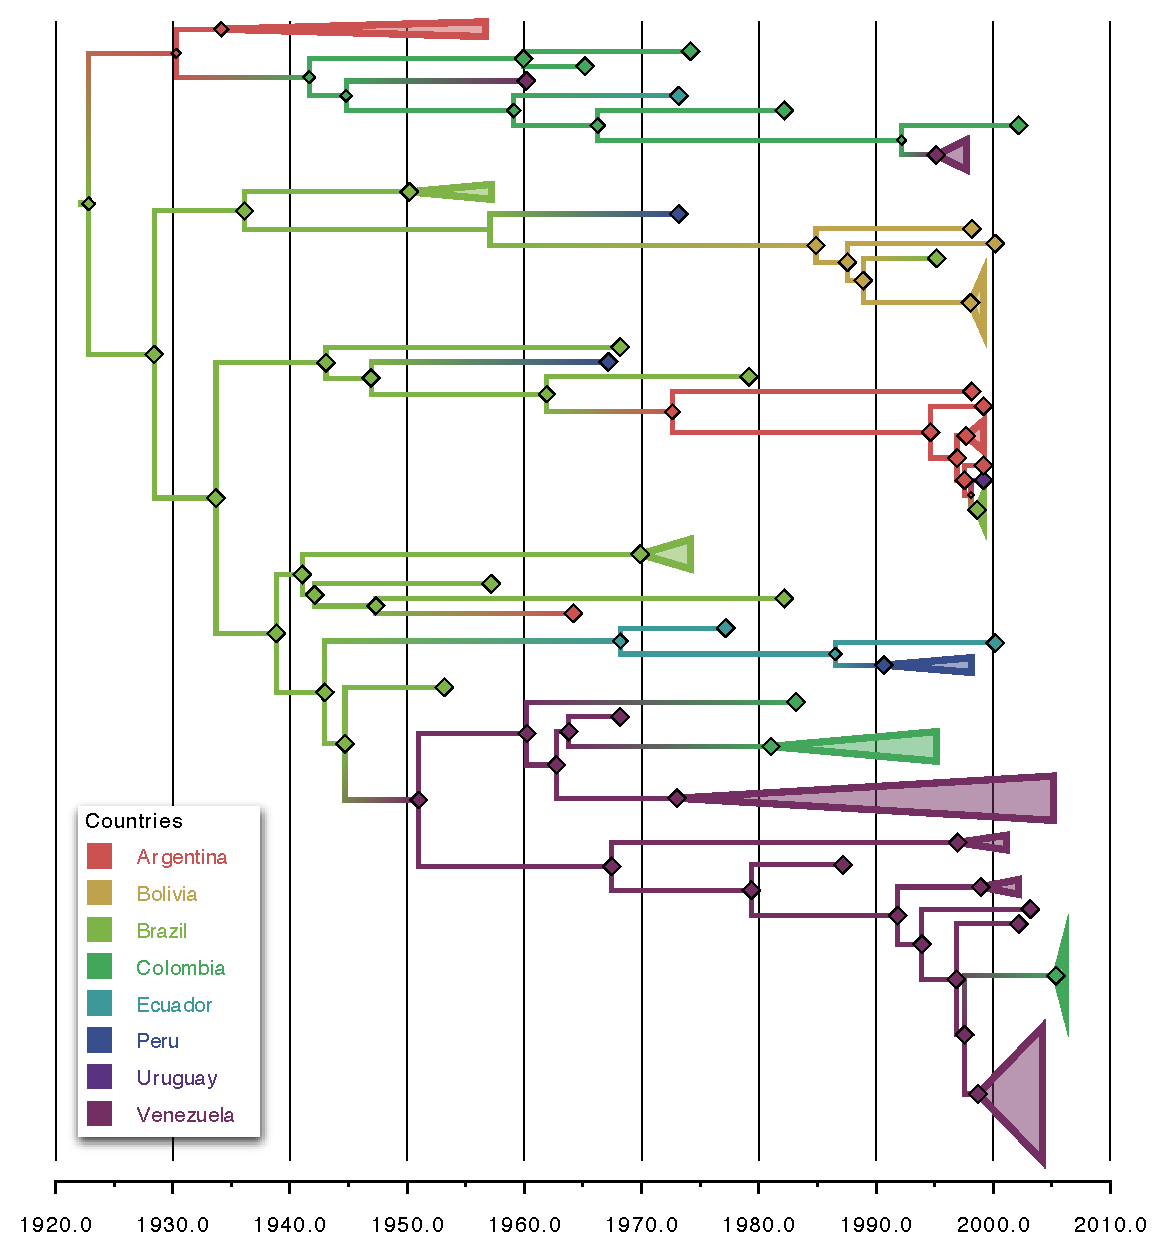
\includegraphics[scale=.45]{FIGURES/A.pdf}}\\
% \subfigure[O]{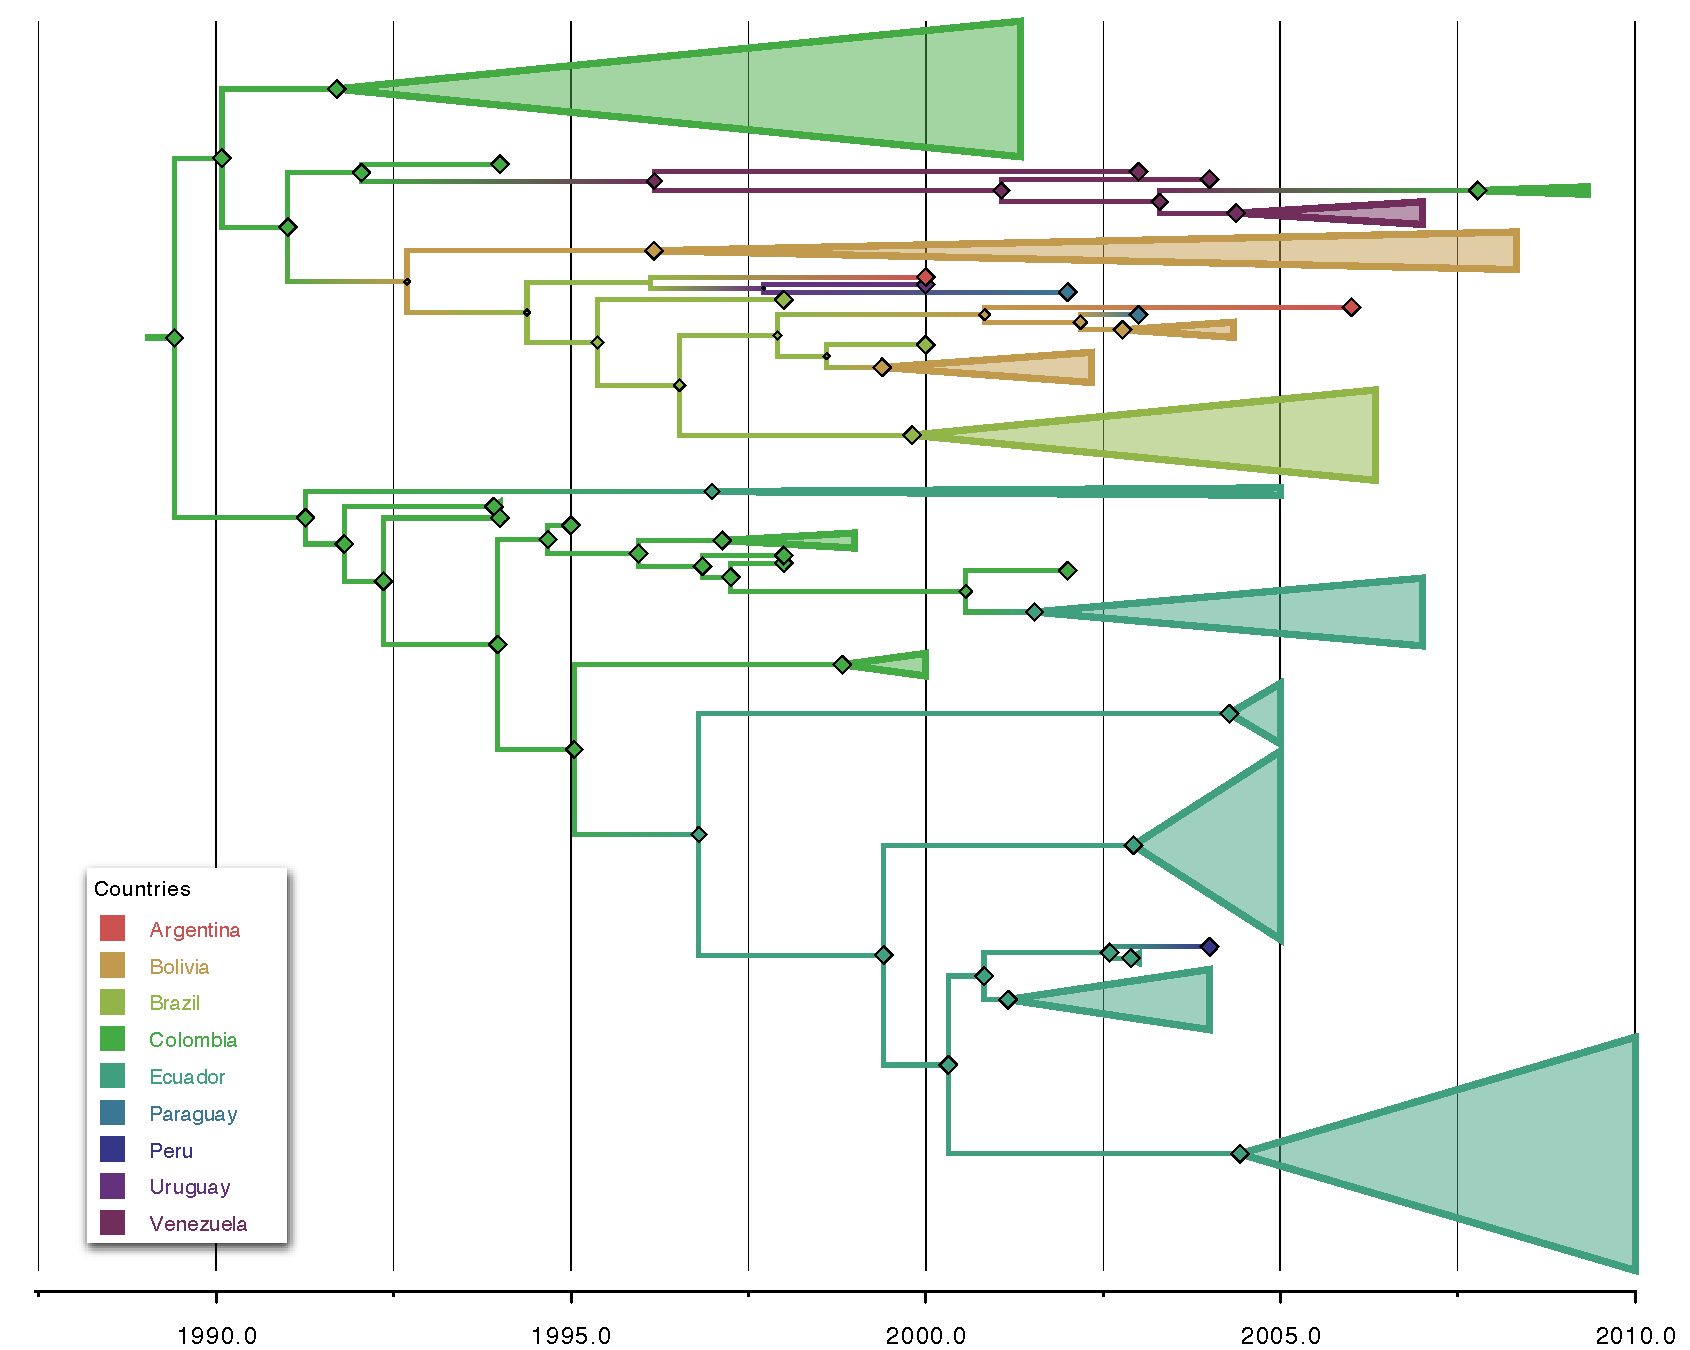
\includegraphics[scale=.30]{FIGURES/O.pdf}}
% \end{center}
% \caption{}
% \label{fig:trees}
% \end{figure}
% %%%%%%%%%%%%%%%%%%%%%%%%%%
% %%%%%%%%%%%%%%%%%%%%%%%%%%
% \begin{table}[H]
% \caption{
% \textbf{.}
% }
% \begin{center}
% \begin{tabular}{lrrrrrr}
% \toprule
%  & \multicolumn{3}{c}{Serotype A}& \multicolumn{3}{c}{Serotype O}\\
%  \midrule
% Predictor & PS & SS & log BF$^2$ & PS & SS & log BF \\
% %\hline
% Cattle&-12588.76&-12591.26&-27.70&\textbf{-8308.94}&\textbf{-8311.21}& \textbf{13.49}\\
% Distance&\textbf{-12557.69}&\textbf{-12559.73}&\textbf{3.83}&-8313.89&-8315.37&9.33\\
% Pigs&-12589.33&-12590.94&-27.38&-8325.39&-8326.63&-1.93\\
% Sheep&-12570.67&-12572.56&-9.00&-8326.23&-8330.64&-5.94\\
% \\
% \hline
% Equal rates &-12561.98&-12563.56&--&-8321.49&-8324.70&--\\
% \bottomrule
% \end{tabular}
% \end{center}
% \begin{flushleft}
% \end{flushleft}
% \label{tab:preds}
%  \end{table}
%%%%%%%%%%%%%%%%%%%%%%%%
\end{document}
